\documentclass[12pt,oneside]{mythesis}
%\includeonly{introduction,conclusion}
\usepackage{algorithmic}
\usepackage{array}
%\usepackage{setspace}
\usepackage[notindex]{tocbibind}
\usepackage{pdflscape}
\usepackage{longtable}
\DeclareMathOperator*{\argmax}{arg\,max}
\usepackage{setspace}
\usepackage{amsmath}
\usepackage{amssymb}
\usepackage{epsfig}
\usepackage{listings}
\usepackage{url}
\usepackage{titlesec}
\usepackage{nameref}
\usepackage[utf8]{inputenc}
\usepackage{mathtools,xparse}
\usepackage{graphicx}
\usepackage{array}
\usepackage{float}
\usepackage{ragged2e}

\usepackage{amsfonts,amsthm}
\usepackage{algorithm2e}
\usepackage{bbm}
% \usepackage[english]{babel}

% set figures directory
\graphicspath{ {figures/} }

\newcommand{\R}{{\mathbb{R}}}
\newcommand{\one}{{\mathbbm{1}}}
\newcommand{\ball}{{\mathrm{B}}}
\newcommand{\fdot}[2]{\langle #1,#2\rangle}
\newtheorem{theorem}{Theorem}
\newtheorem{lemma}{Lemma}
\newtheorem{corollary}{Corollary}

\DeclarePairedDelimiter{\norm}{\lVert}{\rVert}

% fix horizontal and vertical centering
\newcolumntype{P}[1]{>{\centering\arraybackslash}p{#1}}
\newcolumntype{M}[1]{>{\centering\arraybackslash}m{#1}}

\begin{document}

\thispagestyle{empty}
\setlength{\headsep}{0in}
\begin{titlepage}
\centering
\parskip=0pt
\renewcommand{\baselinestretch}{0}
\fontsize{14pt}{0}

\includegraphics[width=1.5in]{kulogo}
\vspace{0.25in}

{\fontsize{0.25in}{0} \textbf{THESIS} }
\vspace{0.38in}

\textbf{BANDIT MULTICLASS LINEAR CLASSIFICATION FOR THE GROUP LINEAR SEPARABLE CASE}
\vfill
\textbf{CHAYUTPONG\ \ PROMPAK}
\vfill
\textbf{GRADUATE SCHOOL, KASETSART UNIVERSITY\\2017}
\vspace{0.15in}
\end{titlepage}
\setlength{\headsep}{0.4in}

% \begin{titlepage}
% \includepdf[noautoscale=true]{approval_scan}
% \end{titlepage}

\begin{titlepage}
\centering
\parskip=\baselineskip
\renewcommand{\baselinestretch}{0}
\fontsize{12pt}{0}
{\fontsize{14pt}{0}\selectfont THESIS}


{\fontsize{14pt}{0}\selectfont BANDIT MULTICLASS LINEAR CLASSIFICATION FOR THE GROUP LINEAR SEPARABLE CASE}
\vfill
CHAYUTPONG\ \ PROMPAK
\vfill
A Thesis Submitted in Partial Fulfillment of \\
the Requirements for the Degree of \\
Master of Engineering (Computer Engineering) \\ 
Graduate School, Kasetsart University \\
2017
\end{titlepage}


\pagenumbering{gobble}
\justify

\newenvironment{indentabstract}[1]%
{\begin{list}{}%
	{\setlength{\leftmargin}{#1}}%
		\item[]%
	}
{\end{list}}

\begin{indentabstract}{0.5in}
Chayutpong Prompak : Bandit Multiclass Linear Classification for The Group
Linear Separable Case. 
Master of Engineering (Computer Engineering), 
Major Field: Computer Engineering, Department of Computer Engineering. 
Thesis Advisor: Assistant Professor
Jittat Fakcharoenphol, Ph.D. Academic Year 2019
\end{indentabstract}
\begin{spacing}{1.75}
\mbox{}
\end{spacing}

We consider the online multiclass linear classification under the
bandit feedback setting.  Beygelzimer, Pal, Szorenyi,
Thiruvenkatachari, Wei, and Zhang [ICML'19] considered two notions
of linear separability, weak and strong linear separability.  When
examples are strongly linearly separable with margin $\gamma$, they
presented an algorithm based on {\sc Multiclass Perceptron} with
mistake bound $O(K/\gamma^2)$, where $K$ is the number of classes.
They employed rational kernel to deal with examples under the weakly
linearly separable condition, and obtained the mistake bound of
\space\space
$\min(K\cdot 2^{\tilde{O}(K\log^2(1/\gamma))},K\cdot
2^{\tilde{O}(\sqrt{1/\gamma}\log K)})$.  In this paper, we refine
the notion of weak linear separability to support the notion of
class grouping, called group weak linear separable condition.  This
situation may arise from the fact that class structures contain
inherent grouping.  We show that under this condition, we can also
use the rational kernel and obtain the mistake bound of $K\cdot
2^{\tilde{O}(\sqrt{1/\gamma}\log L)})$, where $L\leq K$ represents
the number of groups.
\vspace*{\fill}

\noindent\begin{tabular}{c c c}
	\rule{4.2cm}{0.4pt} & \rule{6.5cm}{0.4pt} & 
	\rule{0.8cm}{0.4pt} / \rule{0.8cm}{0.4pt} / \rule{0.8cm}{0.4pt} \\
	Student's signature & Thesis Advisor's signature
\end{tabular}
\justify

\smallskip
{\centering
    \large\bfseries {ACKNOWLEDGEMENTS} \par% copy from command \chaptertitle
}

Mainly, thanks to my advisor Asst. Prof. Dr. Jittat Fakcharoenphol
for lots of help (ie. suggestion, encouragement, teaching).
Thanks to every member of the theory research lab for 
Knowledge, entertainment, fun, and sociability.
Don't miss this one department of computer engineering Kasetsart university 
and official staff involved.

\begin{flushright}
    Chayutpong\space\space Prompak \\
    April 2564
\end{flushright}

\pagenumbering{roman}
\tableofcontents
\clearpage
\listoffigures
\clearpage
% \listoftables
% \clearpage

\pagenumbering{arabic}
\justify

\chaptertitle{INTRODUCTION}
Bandit problems are Sequential decision problems are one model in online learning with has a fixed set of actions, 
(*adversary)
In each round a player pick an action from a set and incur a loss associated with that action.
The goal is to minimize cumulative loss *(at the end).
There are two different observation models depending on information that player received.*(after picked)
In expert case a player knows every losses from every actions in every round.
In bandit case a player knows only the actual losses that picked by a player.
*(measure of interest)
*(weak regret)

*(defination)

background online learning
online learning
sequential decision problems
adversary model
expert , bandit problems
bandit with movement costs
\justify

\chaptertitle{OBJECTIVES}

To extend more specific case that relies on weakly separable case 
and show that the rational kernel can also achieve the spacial case with other variables that make
the mistake boundary to be more suit with the data and find a boundary of the extended case.
\justify

\chaptertitle{LITERATURE REVIEW}

\subsection{Online multiclass classification}
For classification in online version, an input $x_t$ comes at time $t$
, classifier predicts $\hat{y_t}$ then receives feedback information $y_t$ that is the class of $x_t$.
Let $K$ be the number of classes, $T$ be the number of rounds and $y_t\in \ftoN{K}$.
The protocal(fig~\ref{fig:alg-online}) does until time $T$.

\begin{figure}[hbt!]
  \begin{algorithm}[H]
    \SetAlgoLined
    \DontPrintSemicolon
    % \KwData{Number of classes $K$, number of rounds $T$}
    \Begin{
      \For{$t=\ftoN{T}$}{
        Adversary chooses example $(x_t,y_t)\in V \times \ftoN{K}$, where $x_t$ is revealed to the learner.\\
        Predict class label $\hat{y_t} \in \ftoN{K}$.\\
        Observe feedback $y_t$.
        }
        }
        % \caption{{\sc online multiclass classification}\label{alg:online}~\cite{CrammerS2003-ultraconservative}}
      \end{algorithm}
  \centering
  \caption{Online Multiclass Classification Protocal (~\cite{CrammerS2003-ultraconservative})}
  \label{fig:alg-online}
\end{figure}



\subsection{Perceptron}
Perceptron (\cite{rosenblatt58a}) is a binary classifier that answers only input $x$ is in the class or not,
A vector $w$ represented as a class and the answer is depends on the inner product of $x$ and $w$ (fig~\ref{fig:alg-perceptron}).
The perceptron update $w$ only when the answer is wrong 
and makes mistake at most $\left\lfloor \left( \frac{R}{\gamma} \right)^2\right\rfloor$ (theorem~\ref{theorem-perceptron}).

\begin{figure}[hbt!]
  \begin{algorithm}[H]
    \SetAlgoLined
    \DontPrintSemicolon
    \KwData{Number of rounds $T$, $y_t\in \{+1,-1\}$}
    \KwData{Inner product space $(V,\langle\cdot,\cdot\rangle)$}
    \Begin{
      Initialize $w^{(1)}=0$ \\
        \For{$t=\ftoN{T}$}{
          Predict class label $\hat{y_t}
          \begin{cases}
            +1 &\quad \text{if $\langle x_t,w^{(t)}\rangle \geq 0$} \\
            -1 &\quad \text{otherwise}
          \end{cases}
          $.\\
          Observe feedback $y_t$. \;
          \If{$\hat{y_t}\neq y_t$}{
            Update $w^{(t+1)}=w^{(t)}+y_t x_t$ \;
          }
        }
      }
    \end{algorithm}
    \caption{Perceptron Algorithm (~\cite{rosenblatt58a})}
  \label{fig:alg-perceptron}
\end{figure}

\begin{theorem}[~\cite{rosenblatt58a}]
  \label{theorem-perceptron}
  Let $(V,\cdot,\cdot)$ be an inner product space, let $K$ be a
  positive integer, let $\gamma$ be a positive real number and let $R$ be a non-negative real number. If $(x_1,y_1),(x_2,y_2),\dots,(x_K,y_K)$
  is a sequence of labeled examples in $V\times\{+1,-1\}$ and some $\gamma\geq 0$ and
  $\Vert x_1\Vert ,\Vert x_2\Vert ,\dots,\Vert x_T \Vert\leq R$ then PERCEPTRON algorithm makes at most $\left\lfloor \left( \frac{R}{\gamma} \right)^2\right\rfloor$ mistakes.
\end{theorem}

\subsection{Multiclass Perceptron}
Let $K$ be the number of classes, multiclass perceptron construct from $K$ perceptrons
and update depends on $y_t$, see in (fig~\ref{fig:alg-mperceptron}). 
The multiclass perceptron makes mistake at most $\left\lfloor 2\left( \frac{R}{\gamma} \right)^2\right\rfloor$ (theorem~\ref{theorem:mperceptron}).
\begin{figure}[hbt!]
  \begin{algorithm}[H]
    \SetAlgoLined
    \DontPrintSemicolon
    \KwData{Number of classes $K$, number of rounds $T$}
    \KwData{Inner product space $(V,\langle\cdot,\cdot\rangle)$}
    \Begin{
      Initialize $w_1^{(1)}= w_2^{(1)}= \cdots = w_K^{(1)} = 0$ \\
      \For{$t=\ftoN{T}$}{
        Observe feature vector $x_t\in V$.\\
        Predict $\hat{y_t}=\text{argmax}_{i\in \ftoN{K}}\left<w_t^{(i)},x_t\right>$.\\
        Observe $y_t\in\ftoN{K}$.\\
        \eIf{$\hat{y_t}\neq y_t$}{
          Set $w_i^{(t+1)}=w_i^{(t)}$\\
          For all $i\in \ftoN{K}\setminus\{y_t,\hat{y_t}\}$ \;
          Update $w_{y_t}^{(t+1)}=w_{y_t}^{(t)}+x_t$ \;
          Update $w_{\hat{y_t}}^{(t+1)}=w_{\hat{y_t}}^{(t)}-x_t$ \;
        }{
          Set $w_{i}^{(t+1)}=w_{i}^{(t)}$ for all $i\in \ftoN{K}$
        }
      }
    }
  \end{algorithm}
  \caption{Multiclass Perceptron Algorithm (~\cite{CrammerS2003-ultraconservative})}
  \label{fig:alg-mperceptron}
\end{figure}

\begin{theorem}[~\cite{CrammerS2003-ultraconservative}]
\label{theorem:mperceptron}
Let $(V,\cdot,\cdot)$ be an inner product space, let $K$ be a
positive integer, let $\gamma$ be a positive real number and let $R$ be a non-negative real number. If $(x_1,y_1),(x_2,y_2),\dots,(x_K,y_K)$
is a sequence of labeled examples in $V\times\ftoN{K}$ that are strongly linearly separable with margin $\gamma$ and
$\Vert x_1\Vert ,\Vert x_2\Vert ,\dots,\Vert x_T \Vert\leq R$ then MULTICLASS PERCEPTRON algorithm makes at most $\left\lfloor 2\left( \frac{R}{\gamma} \right)^2\right\rfloor$ mistakes.
\end{theorem}


\subsection{Linear seperability}
We restate the definitions for strong and weak linear separability by Beygelzimer~{\em et. al.}~\cite{BeygelzimerPSTWZ2019-separable} here.  
We use the common notation that $[K]=\{1,2,\ldots,K\}$.

\subsubsection{Strongly linear seperable}
The examples lie in an inner product space $(V,\langle\cdot,\cdot\rangle)$.  Let $K$ be the number of classes and let $\gamma$ be a positive real number.
Labeled examples
$(x_1,y_1),(x_2,y_2),\ldots,(x_T,y_T)\in V\times[K]$
are {\em strongly linear separable with margin $\gamma$} if there exist vectors $w_1,w_2,\ldots,w_K\in V$ such that
for all $t\in[T]$,
\[
\langle x_t, w_{y_t}\rangle \geq \gamma/2,
\]
and
\[
\langle x_t, w_i\rangle \leq -\gamma/2,
\]
for $i\in [K]\setminus \{y_t\}$,
and $\sum_{i=1}^K \Vert w_i \Vert^2\leq 1$.
\subsubsection{Weakly linear seperable}
On the other hand, the labeled examples are {\em weakly linear separable with margin $\gamma$} if there exist vectors $w_1,w_2,\ldots,w_K\in V$ such that
for all $t\in[T]$,
\[
\langle x_t, w_{y_t}\rangle \geq \langle x_t, w_i\rangle + \gamma,
\]
for $i\in [K]\setminus \{y_t\}$, and $\sum_{i=1}^K \Vert w_i \Vert^2\leq 1$.

\subsection{Kernel}
We give an overview of the kernel methods (see~\cite{ShaweTaylorC2004-kernel-methods} for expositions) and the rational kernel~\cite{ShalevShwartzSS2011-kernel-based}.

The kernel method is a standard approach to extend linear classification algorithms that use only inner products to handle the notions of ``distance'' between pairs of examples to nonlinear classification.
A {\em positive definite kernel} (or {\em kernel}) is a function of the form $k: X\times X\rightarrow \R$ for some set $X$ such that the matrix $[k(x_i,x_j)]_{i,j=1}^m$ is symmetric positive definite for any set of $m$ examples $x_1,x_2,\ldots,x_m\in X$.  It is known that for every kernel $k$, there exists some inner product space $(V,\fdot{\cdot}{\cdot})$ and a feature map $\phi:X\rightarrow V$ such that $k(x,x')=\fdot{\phi(x)}{\phi(x')}$.  Therefore, a linear learning algorithm can essentially non-linearly map every example into $V$ and work in $V$ instead of the original space without explicitly working with $\phi$ using $k$.  This can be very helpful when the dimension of $V$ is infinite.

As in Beygelzimer~{\em et al.}~\cite{BeygelzimerPSTWZ2019-separable}, we use the rational kernel.  Assume that examples are in $\R^d$.  Denote by $\ball(0,1)$ a unit ball centered at $0$ in $\R^d$.
The {\em rational kernel} $k:B(0,1)\times B(0,1)\rightarrow\R$ is defined as
\[
k(x,x')=\frac{1}{1-\frac{1}{2}\langle x,x'\rangle_{\R^d}}.
\]
Given $x,x'\in\R^d$, $k(x,x')$ can be computed in $O(d)$ time.

Let $\ell_2=\{x\in\R^{\infty} : \sum_{i=1}^\infty x_i^2 < +\infty \}$ be the classical real separable Hilbert space equipped with the standard inner product $\fdot{x}{x'}_{\ell_2}=\sum_{i=1}^\infty x_i x'_i$.  We can index the coordinates of $\ell_2$ by $d$-tuples $(\alpha_1,\alpha_2,\ldots,\alpha_d)$ of non-negative integers, the associated feature map $\phi:\ball(0,1)\rightarrow\ell_2$ to $k$ is defined as
\begin{multline}
\left(\phi(x_1,x_2,\ldots,x_d)\right)_{(\alpha_1,\alpha_2,\ldots,\alpha_d)} =
\\
x_1^{\alpha_1}x_2^{\alpha_2}\cdots x_d^{\alpha_d}
\cdot
\sqrt{2^{-(\alpha_1+\alpha_2+\cdots+\alpha_d)}{{\alpha_1+\alpha_2+\cdots+\alpha_d}\choose{\alpha_1,\alpha_2,\ldots,\alpha_d}}},
\label{eqn:phi}
\end{multline}
where
${{\alpha_1+\alpha_2+\cdots+\alpha_d}\choose{\alpha_1,\alpha_2,\ldots,\alpha_d}}
=
\frac{(\alpha_1+\alpha_2+\cdots+\alpha_d)!}{\alpha_1!\alpha_2!\cdots\alpha_d!}$
is the multinomial coefficient.  It can be verified that $k$ is the
kernel with its feature map $\phi$ to $\ell_2$ and for any
$x\in\ball(0,1)$, $\phi(x)\in\ell_2$.

\subsection{Multiclass Linear Classification}

Beygelzimer~{\em et al.}~\cite{BeygelzimerPSTWZ2019-separable}
presented a learning algorithm for the strongly linearly separable
examples based using $K$ copies of the {\sc Binary Perceptron}.  They
obtained a mistake bound of $O(K(R/\gamma)^2)$ when the examples are
from $\R^d$ with maximum norm $R$ with margin $\gamma$.

Their approach for dealing the weakly linear separable case is to use
the kernel method.  They introduced the {\sc Kernelized Bandit
  Algorithm} (Algorithm~\ref{alg:kernel-bandit}) and proved the
following theorem.

\begin{figure}[bht!]
  
  \begin{algorithm}[H]
    \SetAlgoLined
    \DontPrintSemicolon
    \KwData{Number of classes $K$, number of rounds $T$}
    \KwData{Kernel function $k(\cdot,\cdot)$}
    \Begin{
        Initialize $J_1^{(1)}=J_2^{(2)}=\cdots=J_k^{(k)}=\emptyset$\;
        \For{$t=\ftoN{T}$}{
          Observe feature vector $x_t$\;
          Compute
          $S_t=\left\{i : 1\leq i\leq K, \sum_{(x,y)\in J_i^{(t)}} yk(x,x_t)\geq 0\right\}$\;
          \eIf{$S_t=\emptyset$}{
            Predict $\hat{y}_t\sim \mbox{Uniform}(\{1,2,\ldots,K\})$\;
            Observe feedback $z_t=\one[\hat{y}_t\neq y_t]$\;
            \eIf{$z_t=1$}{
              Set $J_i^{(t+1)} = J_i^{(t)}$ for all $i\in\{1,2,\ldots,K\}$
            }{
              Set $J_i^{(t+1)} = J_i^{(t)}$ for all $i\in\{1,2,\ldots,K\}\setminus\{\hat{y}_t\}$\;
              Update $J_{\hat{y}_t}^{(t+1)}=J_{\hat{y}_t}^{(t)}\cup\{(x_t,+1)\}$
            }
          }{
            Predict $\hat{y}_t\in S_t$ chosen arbitrarily\;
            Observe feedback $z_t=\one[\hat{y}_t\neq y_t]$\;
            \eIf{$z_t=1$}{
              Set $J_i^{(t+1)} = J_i^{(t)}$ for all $i\in\{1,2,\ldots,K\}\setminus\{\hat{y}_t\}$\;
              Update $J_{\hat{y}_t}^{(t+1)}=J_{\hat{y}_t}^{(t)}\cup\{(x_t,-1)\}$
            }{
              Set $J_i^{(t+1)} = J_i^{(t)}$ for all $i\in\{1,2,\ldots,K\}$
            }
          }
        }
      }
    \end{algorithm}
    \caption{Kernelized Bandit Algorithm (~\cite{BeygelzimerPSTWZ2019-separable})}
    \label{alg:kernel-bandit}
\end{figure}

\begin{theorem}[Theorem 4 from~\cite{BeygelzimerPSTWZ2019-separable}]
  Let $X$ be a non-empty set, let $(V,\fdot{\cdot}{\cdot})$ be an
  inner product space.  Let $\phi:X\rightarrow V$ be a feature map and
  let $k:X\times X\rightarrow\R$, where
  $k(x,x')=\fdot{\phi(x)}{\phi(x')}$, be the kernel.  If
  $(x_1,y_1),(x_2,y_2),\ldots,(x_T,y_T)\in X\times\{1,2,\ldots,K\}$
  are labeled examples such that
  \begin{enumerate}
  \item the mapped examples $(\phi(x_1),y_1),\ldots,(\phi(x_T),y_T)$
    are strongly linearly separable with margin $\gamma$,
  \item $k(x_1,x_1),k(x_2,x_2),\ldots,k(x_T,x_T)\leq R^2$
  \end{enumerate}
  then the expected number of mistakes that the {\sc Kernelized Bandit
    Algorithm} makes is at most $(K-1)\lfloor 4(R/\gamma)^2 \rfloor$.
  \label{thm:kernel-bandit-mistake-bound}
\end{theorem}

  The key theorem for establishing the mistake bound is the following
margin transformation theorem based on the rational kernel.

\begin{theorem}[Theorem 5 from~\cite{BeygelzimerPSTWZ2019-separable}]
  (Margin transformation from~\cite{BeygelzimerPSTWZ2019-separable}). Let
  $(x_1,y_1),(x_2,y_2),\ldots,(x_T,y_T)\in \ball(0,1)\times [K]$ be a
  sequence of labeled examples that is weakly linear separable with
  margin $\gamma >0$.  Let $\phi$ defined as in (\ref{eqn:phi}) let
  \[
  \gamma_1 = \frac{
    \left[376\lceil\log_2(2K-2)\rceil\cdot\left\lceil\sqrt{\frac{2}{\gamma}}\right\rceil\right]^{
      \frac{-\lceil\log_2(2K-2)\rceil\cdot
      \left\lceil\sqrt{2/\gamma}\right\rceil}{2}}
  }{2\sqrt{K}},
  \]
  \[
  \gamma_2 =
  \frac{
    \left(2^{s+1}r(K-1)(4s+2)\right)^{-(s+1/2)r(K-1)}
  }{
    4\sqrt{K}(4K-5)2^{K-1}
  }
  \]
  where $r=2\lceil\frac{1}{4}\log_2(4K-3)\rceil+1$ and
  $s=\lceil\log_2(2/\gamma)\rceil$.  Then the feature map $\phi$ makes
  the sequence $(\phi (x_1),y_1),(\phi (x_2),y_2),\ldots,(\phi
  (x_T),y_T)$ strongly linearly separable with margin
  $\gamma'=\max\{\gamma_1,\gamma_2\}$.  Also for all $t$,
  $k(x_t,x_t)\leq 2$.
\end{theorem}

This implies the following mistake bound.
\begin{corollary}[Corollary 6 from~\cite{BeygelzimerPSTWZ2019-separable}]
    (Mistake upper bound
    from~\cite{BeygelzimerPSTWZ2019-separable}). The mistake bound made
    by Algorithm~\ref{alg:kernel-bandit} when the examples are weakly
    linearly separable with margin $\gamma$ is at most
    $\min(2^{\tilde{O}(K\log^2(1/\gamma))},2^{\tilde{O}(\sqrt{1/\gamma}\log
      K)})$.
  \end{corollary}
  
  Beygelzimer {\em et al.}~\cite{BeygelzimerPSTWZ2019-separable} gave two margin transformation proofs.  
  In this paper, we only provide one margin transformation based on the Chebyshev polynomials (Theorem 7 from~\cite{BeygelzimerPSTWZ2019-separable}).

\subsection{Separating polynomials}
\label{sect:sep-poly}

This section proves Theorem~\ref{thm:sep-poly}.  As
in~\cite{BeygelzimerPSTWZ2019-separable}
and~\cite{KlivansS2004-halfspaces-margin}, we use the Chebyshev
polynomials~\cite{MasonH2002-chebyshev} $T_n(\cdot)$ defined as
follows.
\begin{align*}
    T_0(z)&=1,\\
    T_1(z)&=z,\\
    T_{n+1}&=2z T_n(z)-T_{n-1}(z) \;\;\text{for $n\geq 1$}
\end{align*}

The following two lemmas are
from~\cite{BeygelzimerPSTWZ2019-separable}.

\begin{lemma}[from Lemma 15 in~\cite{BeygelzimerPSTWZ2019-separable}]
\label{lem:cheby-prop}
(Properties of Chebyshev polynomials) Chebyshev polynomials satisfy
\begin{enumerate}
    \item $deg(T_n) = n$ for all $n \geq 0$.
    \item If $n \geq 1$, the leading coefficient of $T_n(z)$ is $2^{n-1}$.
    \item $T_n(\cos (\theta)) = \cos (n\theta)$ for all $\theta \in \R$ and all $n \geq 0$.
    \item $T_n(\cosh (\theta)) = \cosh (n\theta)$ for all $\theta \in \R$ and all $n \geq 0$.
    \item $|T_n(z)| \leq 1$ for all $z \in [-1, 1]$ and all $n \geq 0$.
    \item $T_n(z) \geq 1 + n^2(z - 1)$ for all $z \geq 1$ and all $n \geq 0$.
    \item $\|T_n\| \leq (1+\sqrt{2})^n$ for all $n \geq 0$.
\end{enumerate}
\end{lemma}

\begin{lemma}[from Lemma 14 in~\cite{BeygelzimerPSTWZ2019-separable}]
\label{lem:poly-prop}
(Properties of norm of polynomials) 
\begin{enumerate}
    \item Let $p_1,p_2,\ldots,p_n$ be multivariate polynomials and let $p(x)=\prod_{j=1}^n p_j(x)$
    be their product. Then, $\|p\|^2\leq n^{\sum_{j=1}^n deg(p_j)}\prod_{j=1}^n \|p_j\|^2$.
    \item Let $q$ be a multivariate polynomial of degree at most $s$ and let $p(x)=(q(x))^n$. Then,
    $\|p\|^2\leq n^{ns}\|q\|^{2n}$.
    \item Let $p_1,p_2,\ldots,p_n$ be multivariate polynomials. Then, 
    $\left\|\sum_{j=1}^n p_j\right\|^2 \leq n\sum_{j=1}^n \|p_j\|^2.$
\end{enumerate}
\end{lemma}
\justify

\chaptertitle{MATERIALS AND METHODS}
\section{Materials}
\begin{enumerate}
  \item Acer Swift SF314
  \item Logitech G403 hero
  \item SteelSeries QcK mini
  \item AKG N20
\end{enumerate}

\section{Methods}
\subsection{Intra-group boundaries}
We first prove a structural property of intra-group classes.  The
following lemma shows that it is possible to separate one class from
the rest in the same group using only lower and upper thresholds.
This is independent of the number of classes in that group.

\begin{lemma}
  For any group $i\in [L]$, for any class $y\in G_i$, there exists
  reals $b_i\leq t_i$ such that for all $t\in[T]$ such that
  (1) when $y_t=y$, 
  \[
  b_i + \gamma \leq \langle u'_i,x_t\rangle \leq t_i - \gamma;
  \]
  and (2) when $g(y_t)=g(y)$ but $y_t\neq y$, either
  \[
  \langle x_t,u'_i\rangle \leq b_i - \gamma,
  \]
  or
  \[
  \langle x_t,u'_i\rangle \geq t_i + \gamma.
  \]
  \label{lemma:boundaries}
\end{lemma}
\begin{proof}{lemma \ref{lemma:boundaries}}
  Let $S_y = \{(x_j,y_j) : y_j=y, 1\leq j\leq T\}$ be the set of
  examples with label $y$.  Let $b_i=\min_{(x,y)\in S_y}\langle
  x,u'_i\rangle-\gamma$ and $t_i=\max_{(x,y)\in S_y}\langle
  x,u'_i\rangle+\gamma$.  The lemma follows from the definition of
  group weakly linear separability.
\end{proof}

\subsection{Group weakly linear separability}
We now define group weakly linear separability.
Let ${\mathcal G}=\{G_1,G_2,\ldots,G_L\}$ be a partition of $[K]$, i.e., $G_i\subseteq [K]$ for all $i$,
$G_i\cap G_j=\emptyset$ for $i\neq j$, and $\bigcup G_i = [K]$.  
Let $g:[K] \rightarrow [L]$ be a mapping function such that $g(i)\mapsto j$ iff $i\in G_j$.
We say that the labeled examples
$(x_1,y_1),(x_2,y_2),\ldots,(x_T,y_T)\in V\times[K]$
are {\em group weakly linear separable with margin $\gamma$ under ${\mathcal G}$} 
if 
\begin{enumerate}
\item there exist vectors $u_1,u_2,\ldots,u_L\in V$ such that
$\sum_{i=1}^L \Vert u_i \Vert^2\leq 1$, and, for all $t\in[T]$, 
\[
\langle x_t, u_{g(y_t)}\rangle \geq \langle x_t, u_p\rangle + \gamma,
\]
for all $p\in [L] \setminus\{g(y_t)\}$, 
%
\item there exist vectors $u'_1,u'_2,\ldots,u'_L\in V$ such that
$\sum_{i=1}^L \Vert u'_i \Vert^2\leq 1$, and, for all $t\in[T], t'\in[T]$ such that $y_t\neq y_{t'}$ and $g(y_t)=g(y_{t'})$,
either
\[
\langle x_t, u'_{g(y_t)}\rangle \geq \langle x_{t'}, u'_{g(y_t)}\rangle + 2\gamma,
\]
or
\[
\langle x_t, u'_{g(y_t)}\rangle \leq \langle x_{t'}, u'_{g(y_t)}\rangle - 2\gamma.
\]
\end{enumerate}

Note that vectors $u_i$'s define inter-group hyperplanes, while each
$u'_i$ defines intra-group boundaries.  Also note that, to simplify
our proofs, the ``margin'' between intra-group classes is $2\gamma$;
this would create the $+\gamma$ and $-\gamma$ gaps that already exist
between groups.

To illustrate the idea, Fig.~\ref{fig:sep-examples} showing different linear separable conditions.
Thick lines represent class boundaries. 
(a) Strongly linear separable examples with 3 classes (linearly separable in $\R^3$).  
(b) Weakly linear separable examples with 3 classes.  
(c) Group weakly linear separable examples with 3 groups; group 1 (white) contains 3 classes, group 2 (black) contains 4 classes, and group 3 (gray) contains 1 class.  

\begin{figure}[h]
\centering
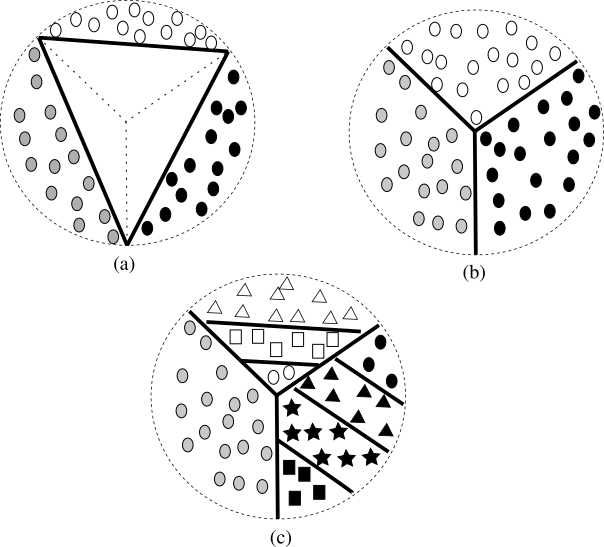
\includegraphics[width=0.45\textwidth]{sep-examples.png}
\caption{Three set of examples in $\R^2$.}
\label{fig:sep-examples}
\end{figure}

\subsection{Margin transformation}

This section is devoted to the proofs of
Theorem~\ref{thm:margin-trans}.  A key property of the space $\ell_2$
is that it contains all multivariate polynomials and the rational
kernel $k$ allows us to work in that space.  The following lemma is
from~\cite{BeygelzimerPSTWZ2019-separable}.

\begin{lemma}[from Lemma 9 in~\cite{BeygelzimerPSTWZ2019-separable}]
\label{lem:norm-bound}
(Norm bound) Let $p:\R^d\to \R$ be a multivariate polynomial. There exists $c\in \ell_2$ such that $p(x)=\fdot{c}{\phi(x)}_{\ell_2}$ and $\|c\|_{\ell_2}\leq 2^{deg(p)/2}\|p\|.$
\end{lemma}

To proof Theorem~\ref{thm:margin-trans}, we need to establish the
existence of multivariate polynomials that separate one class from the
other.  Consider class $i\in [K]$ in group $g(i)$.  Its positive
example $x$, when compared with examples from other group $j\neq
g(i)$, satisfies
\[
\langle u_{g(i)},x\rangle - \langle u_j,x\rangle
=
\langle u_{g(i)}-u_j,x\rangle 
\geq \gamma,
\]
implying that all examples in class $i$ lie in
\[
R^{+}_i = \bigcap_{j\neq g(i)}\{x : \langle u_{g(i)}-u_j,x\rangle \geq \gamma\}, 
\]
while all examples in other groups lie in
\[
R^{-}_i = \bigcup_{j\neq g(i)}\{x : \langle u_{g(i)}-u_j,x\rangle \leq -\gamma\}.
\]
When comparing with other classes $j$ in the same group $g(i)$, from
Lemma~\ref{lemma:boundaries}, we know that there exists thresholds
$b_i$ and $t_i$ that can be used to separate examples from group $i$,
i.e., all its positive examples lie in 
\[
\hat{R}^{+}_i=\{x : \langle u'_{g(i)},x\rangle \geq b_i+\gamma\}
\cap
\{x : \langle u'_{g(i)},x\rangle \leq t_i-\gamma\},
\]
while examples from other classes in group $g(i)$ lie in 
\[
\hat{R}^{-}_i=\{x : \langle u'_{g(i)},x\rangle \leq b_i-\gamma\}
\cup
\{x : \langle u'_{g(i)},x\rangle \geq t_i+\gamma\}.
\]
Let $v_b=\frac{b_i}{\|u'_{g(i)}\|}u'_{g(i)}$ and
$v_t=\frac{t_i}{\|u'_{g(i)}\|}u'_{g(i)}$.  Both sets can be expressed as
\begin{align*}
\hat{R}^{+}_i = & \ 
\{x : \langle u'_{g(i)},x\rangle \geq \langle u'_{g(i)},v_b \rangle+\gamma\} 
\ \cap \\
& \ \{x : \langle u'_{g(i)},x\rangle \leq \langle u'_{g(i)},v_t \rangle-\gamma\},
\end{align*}
while examples from other classes in group $g(i)$ lie in 
\begin{align*}
\hat{R}^{-}_i = & \
\{x : \langle u'_{g(i)},x\rangle \leq \langle u'_{g(i)},v_b \rangle-\gamma\}
\ \cup \\
& \ \{x : \langle u'_{g(i)},x\rangle \geq \langle u'_{g(i)},v_t \rangle+\gamma\}.
\end{align*}

From Lemma~\ref{lem:norm-bound}, for class $i$, it is enough to
establish a multivariate polynomial $p_i$ such that
\begin{align*}
x\in R^{+}_i \cap \hat{R}^{+}_i & \ \ \ \Rightarrow & p_i(x) & \geq \gamma'/2, \\
x\in R^{-}_i \cup \hat{R}^{-}_i & \ \ \ \Rightarrow & p_i(x) & \leq -\gamma'/2.
\end{align*}


This is shown in the Theorem~\ref{thm:sep-poly} below.  This theorem
is fairly technical and is proved in Literature~\ref{sect:sep-poly}

\begin{theorem}
(Polynomial approximation of intersection of halfspaces)
Let $v_1,v_2,\ldots,v_m \in V$ such that $\|v_1\|,\|v_2\|,\ldots,\|v_m\| \leq 1$.
Let $v_b,v_t\in V$ such that $\|v_b\|\leq 1$ and $\|v_t\|\leq 1$.
Let $v' \in V$ such that $\|v'\|\leq 1$.
Let $\gamma \in (0,1)$ and $x \in \ball(0,1)$.
There exists a multivariate polynomial $p:\R^d\to \R$ such that
\begin{enumerate}
\item $p(x) \geq \frac{1}{2}$ for all $x \in \left(\bigcap_{i=1}^m \left\{x: \fdot{v_i}{x}\geq \gamma\right\}\right) \cap \left\{x:\fdot{x}{v'} \geq \fdot{v_b}{v'}+\gamma\right\} \cap \left\{x: \fdot{x}{v'} \leq \fdot{v_t}{v'}-\gamma\right\},$
\item $p(x) \leq -\frac{1}{2}$ for all $x \in \left(\bigcup_{i=1}^m \left\{x: \fdot{v_i}{x}\leq -\gamma\right\}\right) \cup \left\{x: \fdot{x}{v'} \leq \fdot{v_b}{v'}-\gamma\right\} \cup \left\{x: \fdot{x}{v'} \geq \fdot{v_t}{v'}+\gamma\right\},$
\item $deg(p)=\lceil\log_2(2m+4)\rceil\cdot\left\lceil\sqrt{\frac{2}{\gamma}}\right\rceil,$
\item $\|p\|\leq \frac{9}{2}\left[420\lceil\log_2(2m+4)\rceil\cdot\left\lceil\sqrt{\frac{2}{\gamma}}\right\rceil\right]^{\frac{\lceil\log_2(2m+4)\rceil\cdot\left\lceil\sqrt{\frac{2}{\gamma}}\right\rceil}{2}}$
\end{enumerate}

\label{thm:sep-poly}
\end{theorem}

Our proof follows the approach in~\cite{BeygelzimerPSTWZ2019-separable}.

\begin{proof}[Proof of Theorem~\ref{thm:sep-poly}]
Let $r=\lceil\log_2(2m+4)\rceil$ and $s=\left\lceil\sqrt{\frac{2}{\gamma}}\right\rceil$.
Define the polynomial $p:\R^d\to \R$ as
\begin{align*}
    p(x) &= m+\frac{5}{2}-\sum_{i=1}^m (T_s(1-\fdot{v_i}{x}))^r \\
    &-(T_s(1-\fdot{x-v_b}{v'}/2))^r \\
    &-(T_s(1-\fdot{v_t-x}{v'}/2))^r.
\end{align*}

First, consider the case when
\begin{align*}
  x \in & \left(\bigcap_{i=1}^m \left\{x: \fdot{v_i}{x}\geq \gamma\right\}\right) \cap \left\{x: \fdot{x}{v'} \geq \fdot{v_b}{v'}+\gamma\right\} \cap \\
  & \left\{x: \fdot{x}{v'} \leq \fdot{v_t}{v'}-\gamma\right\}.
\end{align*}

Note that $\langle v_i, x\rangle \geq \gamma$ for all $i\in [m]$.
Since $\|x\|\leq 1$ and $\|v_i\|\leq 1$, we have $\fdot{v_i}{x} \in [0,1]$; 
thus, $(T_s(1-\fdot{v_i}{x}))^r \in [-1,1]$.
Consider the terms involving $v_b$ and $v_t$.  Since $\|x\|,\|v_b\|,\|v_t\|\leq 1$, we have that $\|x-v_b\|\leq 2$ and $\|v_t-x\|\leq 2$.  This implies that
$1\geq\fdot{x-v_b}{v'}/2\geq\gamma/2$ and $1\geq\fdot{v_t-x}{v'}/2\geq\gamma/2$; hence,
$(T_s(1-\fdot{x-v_b}{v'}/2))^r\in [-1,1]$ and $(T_s(1-\fdot{v_t-x}{v'}/2))^r\in[-1,1]$.
Therefore,
\[
p(x)\geq m+\frac{5}{2}-m-1-1\geq \frac{1}{2}.
\]

Now consider the case when
\begin{align*}
  x  \in & \bigcup_{i=1}^m \left\{x:\fdot{v_i}{x}\leq -\gamma\right\} \cup \left\{x:\fdot{x}{v'} \leq \fdot{v_b}{v'}-\gamma\right\} \cup \\
  & \left\{x:\fdot{x}{v'} \geq \fdot{v_t}{v'}+\gamma\right\}
\end{align*}
There are two subcases to consider.

{\em Subcase 1:} Suppose that for some $i$, $\fdot{v_i}{x}\leq-\gamma$.  
In this case, $1-\fdot{v_i}{x}\geq 1+\gamma$ and
Lemma~\ref{lem:cheby-prop} (part 6) implies that
\[
  T_s(1-\fdot{v_i}{x}) \geq 1+s^2\gamma \geq 1+2 \geq 2,
\]
and thus, $(T_s(1-\fdot{v_i}{x}))^r\geq 2^r\geq 2m+4$.

Since $T_s(1-\fdot{v_i}{x}))^r \geq -1$ for all $i$, 
$(T_s(1-\fdot{x-v_b}{v'}/2))^r\geq -1$, and $(T_s(1-\fdot{v_t-x}{v'}/2))^r\geq -1$, 
we have that
\begin{align*}
    p(x)&=m+\frac{5}{2}-(T_s(1-\fdot{v_i}{x}))^r \\
    &-\sum_{j\in [m]j\neq i} (T_s(1-\fdot{v_j}{x}))^r \\
    &-(T_s(1-\fdot{x-v_b}{v'}/2))^r \\
    &-(T_s(1-\fdot{v_t-x}{v'}/2))^r \\
    &\leq m+\frac{5}{2}-(2m+4)+(m-1)+2 \leq -\frac{1}{2}.
\end{align*}

{\em Subcase 2:} Consider the other case when for all $i$, $\fdot{v_i}{x} > -\gamma$.
We deal with the case that $\fdot{x}{v'} \leq \fdot{v_b}{v'}-\gamma$.  
The case when $\fdot{x}{v'} \geq \fdot{v_t}{v'}+\gamma$ can be handled similarly.

Since $\fdot{x-v_b}{v'} \leq -\gamma$, we have $1-\fdot{x-v_b}{v'}/2\geq 1 + \gamma/2$.
Lemma~\ref{lem:cheby-prop} (part 6) implies that
\[
  T_s(1-\fdot{x-v_b}{v'}/2)\geq 1+s^2\gamma/2 \geq 1+2/2 \geq 2,
\]
and $(T_s(1-\fdot{x-v_b}{v'}/2))^r\geq 2m+4$.  
Applying the same argument as in Subcase 1, this implies that $p(x)\leq-\frac{1}{2}$.

The degree of $p$ is the maximum degree of the terms $(T_s(1-\fdot{v_i}{x}))^r$, $(T_s(1-\fdot{x-v_b}{v'}/2))^r$, and $(T_s(1-\fdot{v_t-x}{v'})/2)^r$; thus, it is $r\cdot s$.

Finally, we prove the upper bound of norm of $p$. Let $f_i(x)=1-\fdot{v_i}{x}$, 
let $k_b(x)=1-\fdot{x-v_b}{v'}/2$, $k_t(x)=1-\fdot{v_t-x}{v'}/2$.
\[
\|f_i\|^2=1+\|v_i\|^2\leq 1+1=2,
\]
\[
\|k_b\|^2=1+\frac{\|x-v_b\|^2\cdot\|u'\|^2}{2}\leq 1+\frac{4\cdot1}{2}=3
\]
and
\[
\|k_t\|^2=1+\frac{\|v_t-x\|^2\cdot\|u'\|^2}{2}\leq 1+\frac{4\cdot1}{2}=3.
\]

Let $T_s(z)=\sum_{j=0}^s c_j z^j$ be the expansion of $s$-th Chebyshev polynomial.

We first deal with $\|T_s(1-\fdot{v_i}{x})\|^2$.
By lemma~\ref{lem:cheby-prop} and \ref{lem:poly-prop}, $s+1\leq2^s$ for any non-negative integer, we have
% need prop of norm of polynomial
\begin{align*}
    \|T_s(1-\fdot{v_i}{x})\|^2 &= \|T_s(f_i)\|^2 \\
    &=\left\|\sum_{j=0}^s c_j(f_i)^j\right\|^2 \\
    &\leq (s+1)\sum_{j=0}^s\left\| c_j(f_i)^j\right\|^2 \\
    &=(s+1)\sum_{j=0}^s c_j^2\left\|(f_i)^j\right\|^2 \\
    &\leq (s+1)\sum_{j=0}^s c_j^2j^j\left\|f_i\right\|^{2j} \\
    &\leq (s+1)\sum_{j=0}^s c_j^2j^j2^{2j} \\
    &\leq (s+1)s^s2^{2s}\sum_{j=0}^s c_j^2 \\
    &=(s+1)s^s2^{2s}\|T_s\|^2 \\
    &=(s+1)s^s2^{2s}(1+\sqrt{2})^{2s} \\
    &=(s+1)\left(4(1+\sqrt{2})^2s\right)^s \\
    &\leq (8(1+\sqrt{2})^2s)^s \\
    &\leq (47s)^s.
\end{align*}

The other two terms $\|T_s(\fdot{x-v_b}{v'}/2)\|^2$ and $\|T_s(\fdot{v_t-x}{v'}/2)\|^2$ can be analyzed similarly.  We have that
\begin{align*}
    \|T_s(\fdot{x-v_b}{v'}/2)\|^2&=\|T_s(k_b)\|^2 \\
    &=\left\|\sum_{j=0}^s c_j(k_b)^j\right\|^2 \\
    &\leq (s+1)\sum_{j=0}^s c_j^2j^j\left\|k_b\right\|^{2j} \\
    &\leq (s+1)\sum_{j=0}^s c_j^2j^j3^{2j} \\
    &\leq (s+1)s^s3^{2s}\sum_{j=0}^s c_j^2 \\
    &=(s+1)s^s3^{2s}\|T_s\|^2 \\
    &=(s+1)s^s3^{2s}(1+\sqrt{2})^{2s} \\
    &=(s+1)\left(9(1+\sqrt{2})^2s\right)^s \\
    &\leq (9(1+\sqrt{2})^2s)^s \\
    &\leq (105s)^s
\end{align*}
% (105s')^s'
and
\begin{align*}
    \|T_s(\fdot{v_t-x}{v'}/2)\|^2 &= \|T_s(k_t)\|^2 \\
    &=\left\|\sum_{j=0}^s c_j(k_t)^j\right\|^2 \\
    &\leq (105s)^s.
\end{align*}

Finally,
\begin{align*}
    \|p\|&\leq m+\frac{5}{2}+\sum_{i=1}^m\left\|T_s(f_i)^r\right\|
    +\left\|T_s(k_b)^r\right\|+\left\|T_s(k_t)^r\right\| \\
    &=m+\frac{5}{2}+\sum_{i=1}^m\sqrt{\left\|T_s(f_i)^r\right\|^2} \\
    &\ \ \ +\sqrt{\left\|T_s(k_b)^r\right\|^2} +\sqrt{\left\|T_s(k_t)^r\right\|^2} \\
    &\leq m+\frac{5}{2}+\sum_{i=1}^m\sqrt{r^{rs}\left\|T_s(f_i)^r\right\|^{2r}} \\
    &\ \ \ +\sqrt{r^{rs}\left\|T_s(k_b)^r\right\|^{2r}}+\sqrt{r^{rs}\left\|T_s(k_t)^r\right\|^{2r}} \\
    &\leq m+\frac{5}{2}+m r^{rs/2}(47s)^{rs/2}+r^{rs/2}(105s)^{rs/2} \\ 
    &\ \ \ +r^{rs/2}(105s)^{rs/2} \\
    &\leq m+\frac{5}{2}+(m+2)(105rs)^{rs/2}.
\end{align*}
Using the fact that $m\leq\frac{1}{2}2^r$ and $r,s \geq 1$, we then have
\begin{align*}
    \|p\| &\leq m+\frac{5}{2}+(m+2)(105rs)^{rs/2} \\
        &\leq \frac{1}{2}2^r+\frac{5}{2}+\left( \frac{1}{2}2^r +2\right)(105rs)^{rs/2} \\
        &\leq 2\cdot2^r+\frac{5}{2}\cdot 2^r(105rs)^{rs/2} \\
        &= 2^r\left( 2+\frac{5}{2}\right)(105rs)^{rs/2} \\
        &\leq 4^{rs/2}\cdot\frac{9}{2}(105rs)^{rs/2} \\
        &=\frac{9}{2}(420rs)^{rs/2}.
\end{align*}
Substitutions of $r$ and $s$ finish the proof.
\end{proof}

Our main technical result is the following margin transformation using the rational kernel.

\begin{theorem}
(Margin transformation). Let $(x_1,y_1),(x_2,y_2),\ldots,(x_T,y_T)\in \ball(0,1)\times [K]$
be a sequence of labeled examples that is group weakly linear separable with margin $\gamma >0$.
Let $L$ be number of group weakly separable such that $L\leq K.$
Let $\phi$ defined as in (\ref{eqn:phi}) let
\[
    \gamma' = \frac{\left[840\lceil\log_2(2L+2)\rceil\cdot\left\lceil\sqrt{\frac{2}{\gamma}}\right\rceil\right]^{-\frac{\lceil\log_2(2L+2)\rceil\cdot\left\lceil\sqrt{\frac{2}{\gamma}}\right\rceil}{2}}}{9\sqrt{L}},
\]
The feature map $\phi$ makes the sequence $(\phi (x_1),y_1),(\phi (x_2),y_2),\ldots,(\phi (x_T),y_T)$
strongly linearly separable with margin $\gamma'$.
\label{thm:margin-trans}
\end{theorem}

We note that the margin depends on $L$, the number of groups, instead of $K$, the number of classes.  Using Theorem~\ref{thm:margin-trans} with Theorem~\ref{thm:kernel-bandit-mistake-bound} we obtain the following mistake bound for our algorithm.

\begin{proof}[Proof of Theorem~\ref{thm:margin-trans}]

Consider class $i\in[K]$. We will apply
Theorem~\ref{thm:sep-poly}. For $j\in\{1,\ldots,L-1\}$, let
\[
v_j=\left\{
\begin{array}{ll}
    u_{g(i)}-u_j, & \mbox{if $j<g(i)$,} \\
    u_{g(i)}-u_{j+1}, & \mbox{if $j>g(i)$.}
\end{array}
\right.    
\]
Also, let $v'=u'_{g(i)}$, $v_b=\frac{b_i}{\|u'_{g(i)}\|}u'_{g(i)}$
and $v_t=\frac{t_i}{\|u'_{g(i)}\|}u'_{g(i)}$.

From Theorem~\ref{thm:sep-poly}, there exists a multivariate
polynomial $p_i:\R^d\to \R$ such that for all $t\in[T]$ and the
sequence $(x_1,y_1),(x_2,y_2),(x_t,y_t),\ldots,(x_T,y_T)$, we have
\begin{itemize}
\item if $y_t=i$, $p_i(x_t)\geq \frac{1}{2}$, since $x_t\in R^{+}_i
    \cap \hat{R}^{+}_i$, and
\item if $y_t\neq i,$ $p_i(x_t)\leq -\frac{1}{2}$, since $x_t\in
    R^{-}_i \cap \hat{R}^{-}_i$.
\end{itemize}

It is left to check the properties of $p$.
Theorem~\ref{thm:sep-poly} implies that
\[
\|p\|\leq \frac{9}{2}\left[420\lceil\log_2(2L+2)\rceil\cdot\left\lceil\sqrt{\frac{2}{\gamma}}\right\rceil\right]^{\frac{\lceil\log_2(2L+2)\rceil\cdot\left\lceil\sqrt{\frac{2}{\gamma}}\right\rceil}{2}}
\]
By Lemma~\ref{lem:norm-bound}, there exists $c_i\in\ell_2$ such that $\fdot{c_i}{\phi(x)}=p_i(x),$ and
\[
\|c_i\|_{\ell_2}\leq \frac{9}{2}\left[840\lceil\log_2(2L+2)\rceil\cdot\left\lceil\sqrt{\frac{2}{\gamma}}\right\rceil\right]^{\frac{\lceil\log_2(2L+2)\rceil\cdot\left\lceil\sqrt{\frac{2}{\gamma}}\right\rceil}{2}}.
\]

We are ready to construct strongly separable vectors for our group
weakly separable case in $\ell_2$ such that
$\|z_1\|^2+\|z_2\|^2+\ldots+\|z_L\|^2\leq 1$ and for all $t\in [T]$,
$\fdot{z_{y_t}}{x_t} \geq \gamma$, and for all $j\neq y_t$,
$\fdot{z_j}{x_t}\leq -\gamma$, by scaling $c_i$ appropriately as
follows.  We can let
\[
z_i=\frac{c_i}{\sqrt{L}\cdot \frac{9}{2}\left[840\lceil\log_2(2L+2)\rceil\cdot\left\lceil\sqrt{\frac{2}{\gamma}}\right\rceil\right]^{\frac{\lceil\log_2(2L+2)\rceil\cdot\left\lceil\sqrt{\frac{2}{\gamma}}\right\rceil}{2}}},
\]
and
\[
\gamma = \frac{\left[840\lceil\log_2(2L+2)\rceil\cdot\left\lceil\sqrt{\frac{2}{\gamma}}\right\rceil\right]^{-\frac{\lceil\log_2(2L+2)\rceil\cdot\left\lceil\sqrt{\frac{2}{\gamma}}\right\rceil}{2}}}{9\sqrt{L}},
\]
then the theorem follows.    
\end{proof}

\begin{corollary}
(Mistake bound for group weakly linearly separable case) 
Let $K$ be positive integer, $L\leq K$ and $\gamma$ be positive real number. 
The mistake bound made by Algorithm~\ref{alg:kernel-bandit} when the examples are group weakly
linearly separable with margin $\gamma$ with $L$ groups is at most
$K\cdot 2^{\tilde{O}(\sqrt{1/\gamma}\log L)}$.
\label{cor:mistake-bound}
\end{corollary}

Note that multiplicative factor of $K$ is hidden from the second bound of~\cite{BeygelzimerPSTWZ2019-separable} because of the $\tilde{O}$ notation on the exponent.  We cannot do that because in our exponent we have only $\log L$ which can be much smaller than $K$.  Their actual bound (showing $K$), which can be compared to ours, is $K\cdot 2^{\tilde{O}(\sqrt{1/\gamma}\log K)}$.
  
\justify

\chaptertitle{EXPERIMENTS}


\justify

\chaptertitle{CONCLUSION AND RECOMMENDATION}

\section{Conclusion}
We prove that mistakes bound of rational kernel in 
group weakly linear separable case is converged up to group number.
\begin{enumerate}
    \item Rational kernel can archives group weakly linear separable case with
$$
\gamma = \my_gamma
$$.
    \item Kernelized Bandit Algorithm makes 
$$
K\cdot 2^{\tilde{O}(\sqrt{1/\gamma}\log L)}
$$
mistakes in group weakly separable case.
    \item If there is no group in a weakly separable case our boundary is as same as
\cite{BeygelzimerPSTWZ2019-separable}
\end{enumerate}

\section{Recommendations}

Notice that the rational kernel is the inner product in infinite dimension space
that can have a lot of vectors in Hilbert space that makes $\gamma$ smaller.
Can we state a separable case that more generally than a weakly separable case?
The boundary is quite loose but this is already very difficult to figure out, 
Can we find another kernel that is easier to analyze?
\chaptertitle{CURRICULUM VITAE}
\noindent\begin{tabbing}
\hspace{1.2in} \= \hspace{2in} \= \kill
\bf{NAME} \> : Chayutpong Prompak \\
\hspace{1in} \\
\bf{BIRTH DATE} \> : July 29, 1993 \\
\hspace{1in} \\
\bf{BIRTH PLACE} \> : Loei, Thailand \\
\hspace{1in} \\
\hspace{1.2in} \= \hspace{1in} \= \hspace{1.5in} \= \hspace{1in} \= \kill
\bf{EDUCATION} \> \underline{\bf{:YEAR}} \> \underline{\bf{INSTITUTE}} \> \underline{\bf{DEGREE/DIPLOMA}} \\
\> 2012 \> Kasetsart Univ. \> B.Eng.(Computer)
\hspace{1in} \\
\hspace{1in} \\
\hspace{2in} \= \hspace{2in} \= \kill
\bf{POSITION/TITLE} \> : - \\
\bf{WORK PLACE} \> : - \\
\bf{SCHOLARSHIP/AWARDS} \> : - \\
\end{tabbing}

\label{ch:cited}
\nocite{*}
% \addcontentsline{toc}{chapter}{\bibname}
% \bibliographystyle{plainnat}
\bibliographystyle{myplainnat}
\bibliography{ref}

\end{document}
